\section{D2L Brightspace}
\subsection{Overview}
Brightspace is a cloud based LMS developed by the software company Desire to Learn (D2L). Its design philosophy is one of flexibility, with the primary goal being to allow every student to study in a way which most benefits them. Brightspace is targeted towards primary and high schools, universities, and corporate learning environments. It offers key features expected of an LMS such as:
\begin{itemize}
  \item Importing and exporting course contents to and from other SCORM compliant LMS's.
  \item Easy management of course contents and resources from the courses page.
  \item Full suite of tools to create assignments, exams and quizzes.
  \item Comprehensive and fully features mobile services.
  \item Organisation features for students and teachers such as calendars and reminders.
\end{itemize}
\cite{brightspaceLMS}

\subsection{Course Management and Contents}
The UI provided by Brightspace for managing and updating courses and their contents is highly simplistic and intuitive, while still allowing administrators to have a high level of control over every aspect of a course. From within a course page, an instructor or administrators can manage contents such as lectures, assignments and quizzes in terms of modules and sub-modules, with the idea that each module is for a specific topic or idea. These modules can be linked to learning outcomes from a rubric, and can be made visible or invisible to specific groups of students within a course.\\ 
From within these course pages, instructors and administrators can also view enrollments, grade-books, and have the ability to quickly view any student submissions that require their attention, both on a course by course view or as a combination of submissions from all courses they manage. From the course page, instructors and administrators can also manage the calendar, forum, and attendance modules for that course.

\begin{figure}
\centering
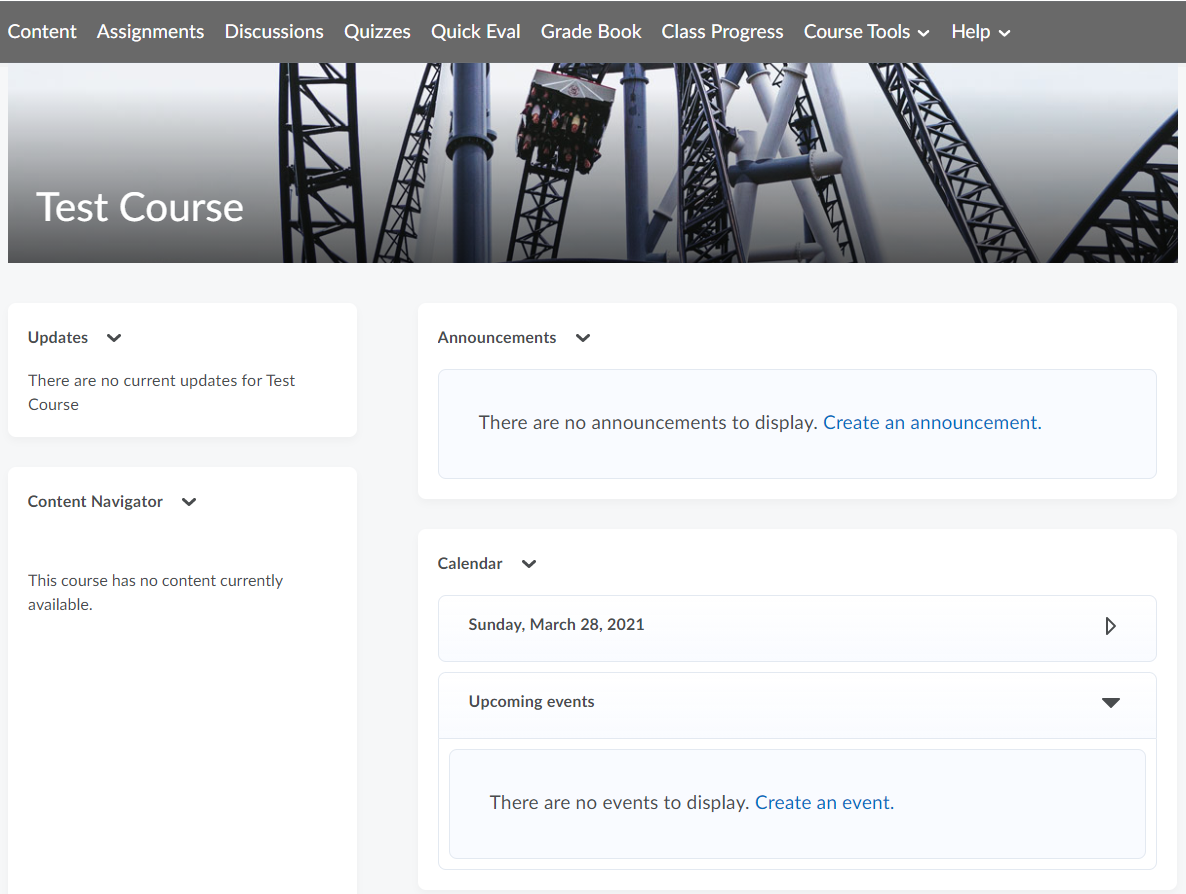
\includegraphics[scale=0.5]{brightspace-dashboard}
\caption{The course dashboard from an instructor's perspective.}
\end{figure}

\subsection{Accounts and Enrollment}
Brightspace gives the option for a course administrator to allow a course to either be built with automatic enrollment, where administrators and instructors enrol students into the course, self enrollment, where students can enroll themselves either by entering a course code or searching for a publicly viewable course, or as a combination of both, where a course can have a number of spaces assigned to each method of enrollment.

\begin{figure}
\centering
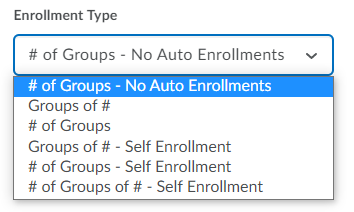
\includegraphics[scale=0.5]{brightspace-enrollment}
\caption{The ability to allow groups of students to either self enroll or be enrolled by an administrator.}
\end{figure}

\subsection{Data migration}
D2L Brightspace provides very robust features to import and export course content, and is SCORM 1.2 and SCORM 2004 compliant. These tools allow course administrators to export course components as a Brightspace package, for use on other Brightspace sites, as well as Common Cartridge and Thin Common Cartridges for exporting modules to other LMS's who also follow the Common Cartridge standard such as Moodle and Canvas.\\
In terms of importing, Brightspace allows administrators to import archived course content from Brightspace itself, as well as other common LMS' such as Angel Learning, Blackboard Learn, Moodle and Sakai, as well as course content compiled according to industry standards including IMS Content Packaging, IMS Common Cartridge, IMS Thing Common Cartridge, and SCORM. It also allows importing of courses and course materials from an online Learning Object Repository (LOR) of hundreds of publicly available courses.\\

\begin{figure}
\centering
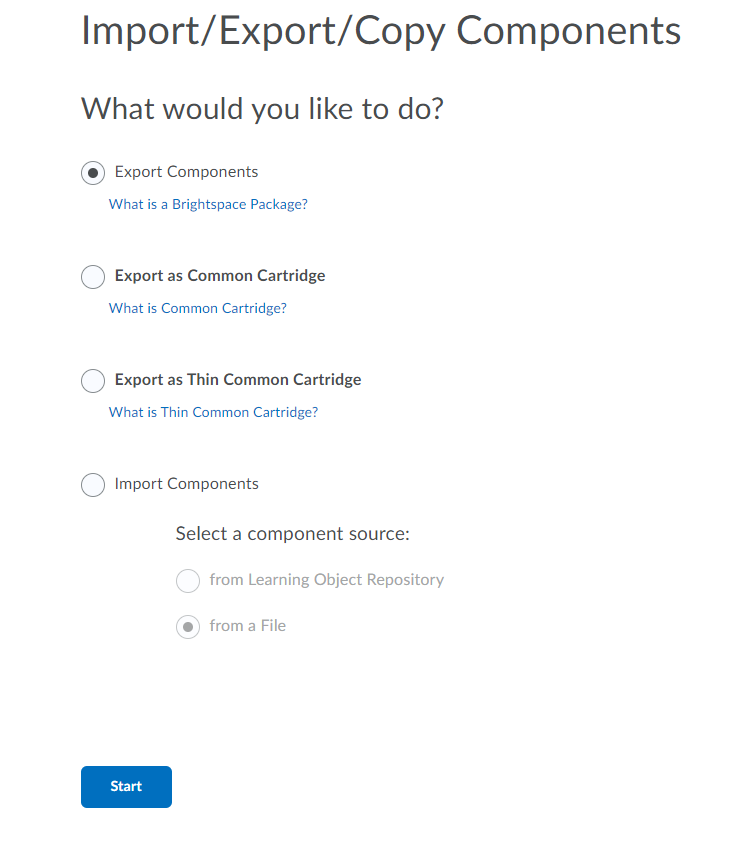
\includegraphics[scale=0.5]{brightspace-export}
\caption{Options to import/export a course on Brightspace.}
\end{figure}

\newpage

\subsection{Conclusion}
Brightspace delivers a responsive, well designed and fully fleshed out LMS experience with great ease-of-use and compatibility with other SCORM and IMS compliant LMS's, with the primary negative being its cost and lack of open source.